\documentclass[aspectratio=169]{beamer}


\usepackage[utf8]{inputenc}
\usepackage{amsmath}
\usepackage{amsfonts}
\usepackage{amssymb}
\usepackage{xcolor}
\usepackage{graphicx}
\usepackage{ragged2e}  % `\justifying` text
\usepackage{booktabs}  % Tables
\usepackage{tabularx}
\usepackage{tikz}      % Diagrams
\usetikzlibrary{calc, shapes, backgrounds}
\usepackage{amsmath}
\usepackage{amssymb}
\usepackage{dsfont}
\usepackage{url, soul}       % `\url
\usepackage{listings}  % Code listings
\usepackage[T1]{fontenc}
\usepackage{multirow}
\usepackage{theme/beamerthemehbrs}

\author[Veeramacheneni]{Lokesh Veeramacheneni}
\title{Out-of-Distribution Detection in 3D Semantic Segmentation}
\subtitle{Master Thesis}
\institute[HBRS]{Hochschule Bonn-Rhein-Sieg}
\date{September 02, 2022}
\subject{Test beamer}

% leave the value of this argument empty if the advisors
% should not be included on the title slide
\def\advisors{Prof. Dr Paul G Ploeger, Prof. Dr Matias Valdenegro Toro, Prof. Dr Sebastian Houben}

\thirdpartylogo{images/DFKI.png}


\begin{document}
{
\begin{frame}
\titlepage
\end{frame}
}

%%%%%%%%%%%%%%%%%%%%%%%%%%%%%%%%%%%%%%%%%%%%%%%%%%%%%%%%%%%%%%%%%%%%%%%%%%%%%%%%%%%%%%%%
%%%%%%%%%%%%%%%%%%%%%%%        Introduction           %%%%%%%%%%%%%%%%%%%%%%%%%%%%%%%%%%
%%%%%%%%%%%%%%%%%%%%%%%%%%%%%%%%%%%%%%%%%%%%%%%%%%%%%%%%%%%%%%%%%%%%%%%%%%%%%%%%%%%%%%%%
\section{Introduction}
% 1. Discuss about what is OOD
% and need for OOD along with some real life examples
% 2. Explain about 3D Semantic segmentation task
\begin{frame}{Out-of-Distribution detection}
    \begin{columns}
        \begin{column}{0.5\textwidth}
            \begin{itemize}
                \item Tesla autonomous driving system detects the Moon as yellow traffic light
                \item These faulty predictions might result in unpredictable behaviour
                \item An ideal trustworthy visual recognition system
                \begin{itemize}
                    \item Produce accurate predictions on known samples
                    \item Detect and reject unknown samples
                \end{itemize}
            \end{itemize}
        \end{column}
        \begin{column}{0.5\textwidth}
            
        \begin{figure}
            \centering
            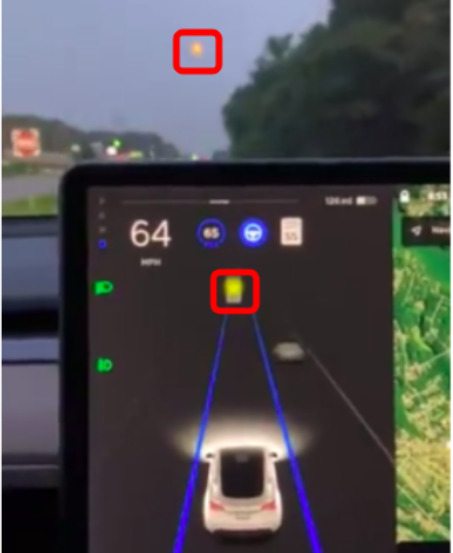
\includegraphics[scale=0.25]{images/Tesla_ex_moon.jpg}
            \caption{Misdetection of Moon as yellow signal light in Tesla driving platform. Image taken from \cite{tesla_fails}.}
            \label{fig:eg_tesla_moon}
        \end{figure}
        \end{column}
    \end{columns}
\end{frame}

\begin{frame}{Out-of-Distribution detection}
    \begin{itemize}
        \item Deep Neural Networks (DNNs) are trained based on closed world assumption
        \item Closed world assumption - test data is assumed to be drawn from same distribution as \textbf{training data} which is called \textbf{In-Distribution (ID)}
        \item When deployed in real-world (\textbf{open world scenario}) these OOD samples can be \textbf{Out-of-Distribution (OOD)}, the test samples can be
        \begin{itemize}
            \item from different class
            \item from different domain 
        \end{itemize}
        %\item Moon is classified as an OOD object in the above example
    \end{itemize}
\end{frame}
\begin{frame}{Importance of OOD detection}
    \begin{columns}
       \begin{column}{0.5\textwidth}
        \begin{itemize}
            \item Figure~\ref{fig:eg_apollo_pipeline} depicts the pipeline of modules in Apollo driving platform
            \item Prediction and motion planning module are dependent on perception module
            \item A misdetection of an OOD sample will propagate the error to motion planning
            \item This error affects the total vehicle control and might lead to unfortunate consequences
        \end{itemize}
       \end{column}
       \begin{column}{0.5\textwidth}
            \begin{figure}
                \centering
                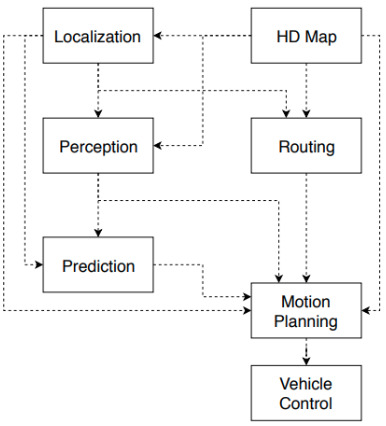
\includegraphics[scale=0.35]{images/apollo_pipeline.jpg}
                \caption{Module pipeline for Apollo autonomous driving platform. Image taken from \cite{baiduapollo}.}
                \label{fig:eg_apollo_pipeline}
            \end{figure}
       \end{column}
    \end{columns}
\end{frame}
\begin{frame}{3D Light Detection And Ranging (LiDAR)}
    \begin{columns}
       \begin{column}{0.5\textwidth}
            \begin{itemize}
                \item Uses \textbf{pulsed lasers} to find the  \textbf{range} to the objects
                \item Unlike images, LiDAR is insusceptible to illumination and provide rich 3D information.
                %\item Figure~\ref{fig:sample_lidar_pc} depicts the sample point cloud with LiDAR is placed in round white circle found at the centre of point cloud
                \item Typically, features of each point in point cloud includes 
                \begin{itemize}
                    \item Spatial features (XYZ)
                    \item Colour (RGB)
                    \item Intensity
                \end{itemize}
            \end{itemize}
       \end{column}
       \begin{column}{0.5\textwidth}
            \begin{figure}
                \centering
                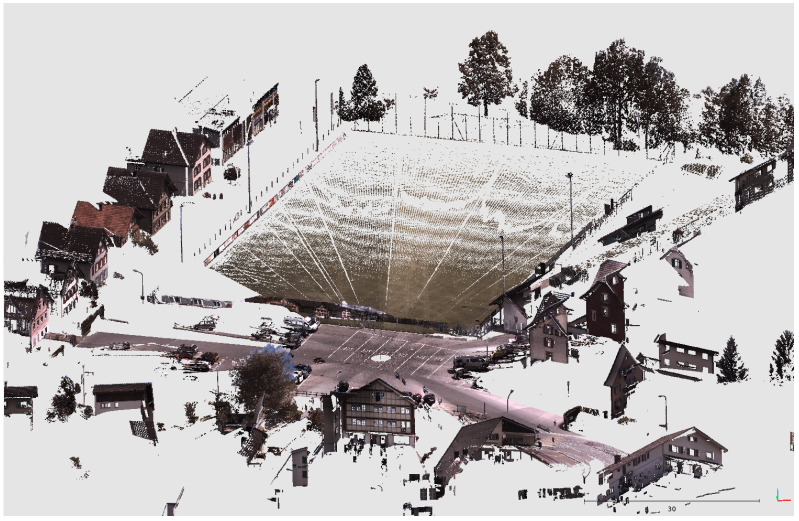
\includegraphics[scale=0.25]{images/sample_LiDAR_PC.jpg}
                \caption{Sample LiDAR point cloud collected in a outdoor scene. Image taken from \cite{hackel2017semantic3d}.}
                \label{fig:sample_lidar_pc}
            \end{figure}
       \end{column}
    \end{columns}
\end{frame}
\begin{frame}{3D Semantic Segmentation}
    \begin{columns}
       \begin{column}{0.4\textwidth}
            \begin{itemize}
                \item An important task in computer vision because of its use in scene understanding
                \item Further helps in navigation and planning of robots
                \item Objective - Assign \textbf{each point} in the point cloud a \textbf{specific class}
            \end{itemize}       
       \end{column}
       \begin{column}{0.6\textwidth}
            \begin{figure}
                \centering
                %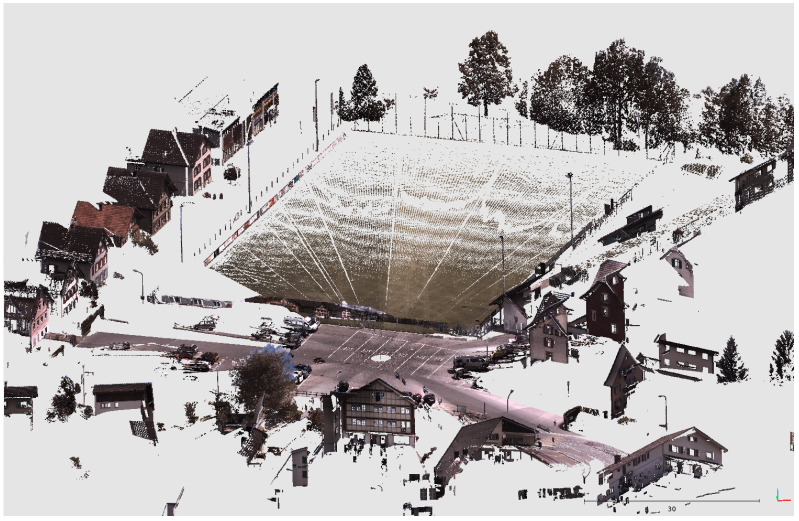
\includegraphics[scale=0.15]{images/sample_LiDAR_PC.jpg}
                %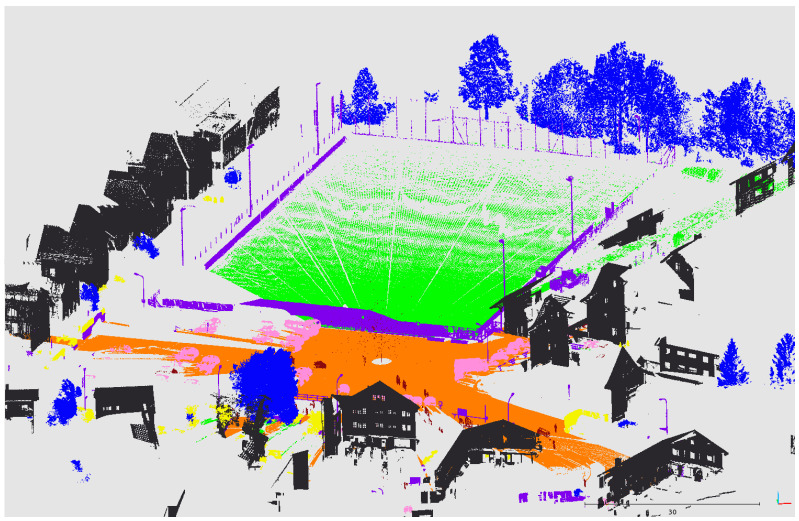
\includegraphics[scale=0.15]{images/sample_LiDAR_PC_segmented.jpg}
                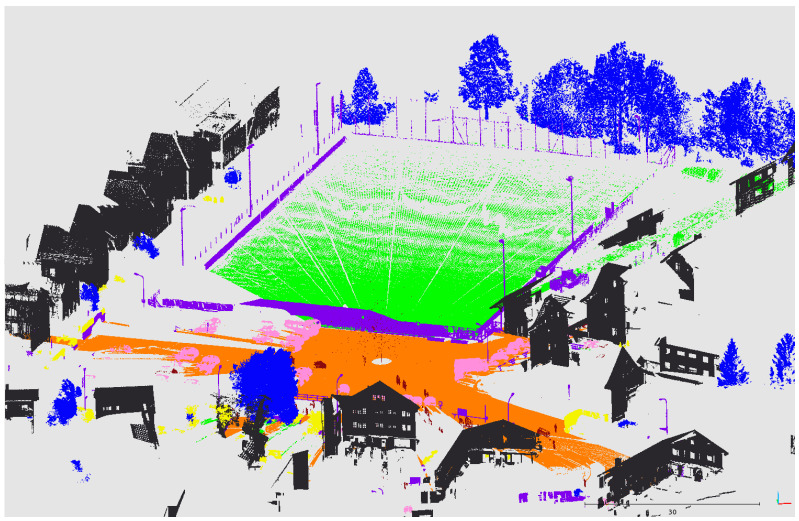
\includegraphics[scale=0.3]{images/sample_LiDAR_PC_segmented.jpg}
                \caption{Segmented output of sample point cloud. Image taken from \cite{hackel2017semantic3d}.}
                \label{fig:sample_lidar_pc_segmented}
            \end{figure}
       \end{column}
    \end{columns}
\end{frame}

\begin{frame}{Thesis objective}

\begin{itemize}
    \item OOD detection in the 3D semantic segmentation setting
    \item Create \textbf{benchmark datasets} for OOD detection among existing 3D LiDAR datasets. We define OOD data based on two categories
    \begin{itemize}
        \item if the point is from different class than training data
        \item if the point has inferior quality
    \end{itemize}
    \item We also study whether \textbf{uncertainty estimation} is a practical approach for OOD detection in 3D domain
\end{itemize}
    
\end{frame}
%%%%%%%%%%%%%%%%%%%%%%%%%%%%%%%%%%%%%%%%%%%%%%%%%%%%%%%%%%%%%%%%%%%%%%%%%%%%%%%%%%%%%%%%
%%%%%%%%%%%%%%%%%%%%%%%        Methodology           %%%%%%%%%%%%%%%%%%%%%%%%%%%%%%%%%%%
%%%%%%%%%%%%%%%%%%%%%%%%%%%%%%%%%%%%%%%%%%%%%%%%%%%%%%%%%%%%%%%%%%%%%%%%%%%%%%%%%%%%%%%%
\section{Experimental Setup \& Methodology}
% Explain about what are the requirements for setup one by one such as
% Datasets & benchmarking, OOD method, 3D Model, Uncertainty methods, Evaluation metrics
\begin{frame}[noframenumbering]{Setup}
    \begin{itemize}

        \item 3D Semantic Segmentation model
        \item Uncertainty methods
        \item OOD score methods
        \item Datasets
    \end{itemize}
\end{frame}
\begin{frame}{RandLA-Net}
    \begin{columns}
        \begin{column}{0.6\textwidth}
            \begin{itemize}
                \item Lightweight, efficient computation, memory usage and inputs 3D point cloud directly
                \item \textbf{Random point sampling} and \textbf{local feature aggregation module} are most important modules
                \item Local feature aggregation module is subdivided into local spatial encoding, attentive pooling and dilated residual block
                \item \textbf{Encoder-Decoder style} architecture as depicted in Figure~\ref{fig:randla_model}
            \end{itemize}
        \end{column}
        \begin{column}{0.4\textwidth}
            \begin{figure}
                \centering
                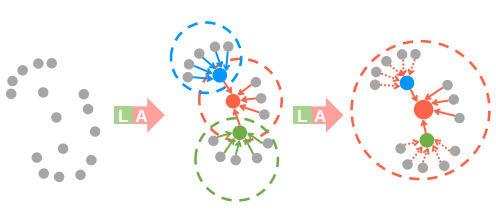
\includegraphics[scale=0.35]{images/randlanet_dires_effect.jpg}
                \caption{Image depicting the working of Dilated residual block with each circle representing the receptive
                field of the block for feature extraction. LA represents the combination of Local Spatial Encoding and
                Attentive Pooling modules combined. Image taken from \cite{Hu_2020_CVPR_Randla}.}
                \label{fig:dires_effect}
            \end{figure}
        \end{column}
    \end{columns}
    
\end{frame}
\begin{frame}{RandLA-Net}
    \begin{figure}
        \centering
        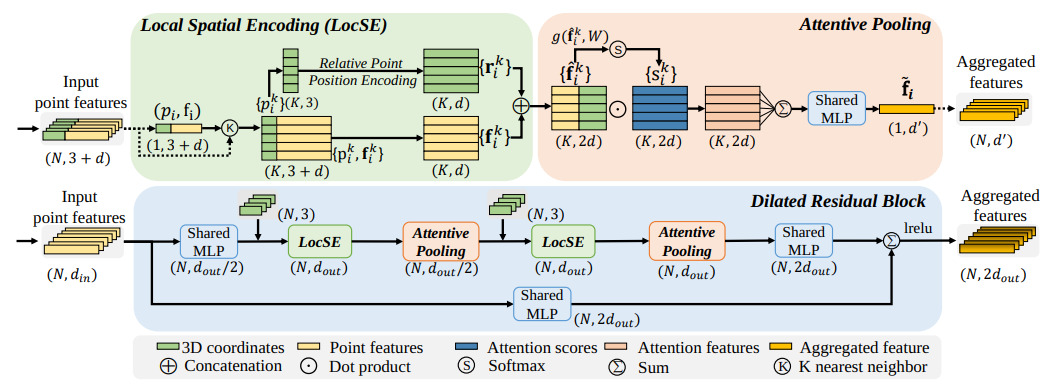
\includegraphics[width = 0.9\textwidth, height=0.37\textheight]{images/randlanet_dires_block.jpg}
        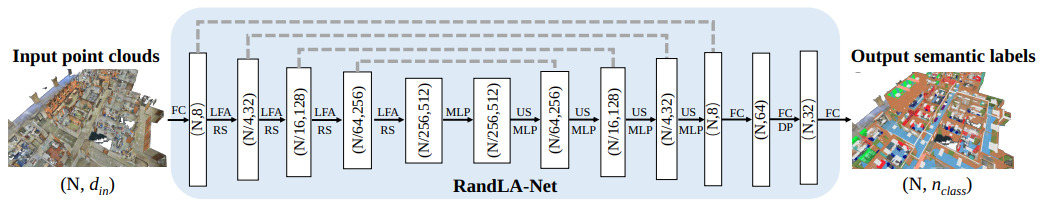
\includegraphics[width = 0.9\textwidth, height=0.37\textheight]{images/randlanet_model.jpg}
        \caption{Illustration of local feature aggregation module in RandLa-Net in top image and architecture of
        RandLA-Net in bottom image. Both the images are taken from \cite{Hu_2020_CVPR_Randla}.}
        \label{fig:randla_model}
    \end{figure}
\end{frame}
\begin{frame}[noframenumbering]{Setup}
    \begin{itemize}
        
        \item \textcolor{gray}{3D Semantic Segmentation model - RandLA-Net}
        \item Uncertainty methods
        \item OOD score methods
        \item Datasets
    \end{itemize}
\end{frame}
\begin{frame}{Deep Ensembles}
    \begin{columns}
        \begin{column}{0.5\textwidth}
            \begin{itemize}
                \item Ensemble learning technique - train N randomly initialized models with same data
                \item Resulting N predictions are then averaged
                \item \textbf{Performance boosting} along with uncertainty value for a prediction
                \item Requires \textbf{more computation power}
            \end{itemize}
        \end{column}
        \begin{column}{0.5\textwidth}
            \begin{figure}
                \centering
                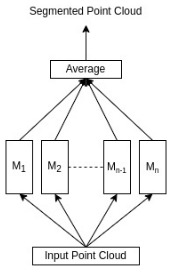
\includegraphics[scale=0.5]{images/deep_ensembles.jpg}
                \caption{Illustration of test dataflow in Deep Ensembles, where input point cloud is fed into multiple
                randomly initialized models $M_1$ to $M_n$.}
                \label{fig:deep_ensembles_work}    
            \end{figure}
        \end{column}
    \end{columns}
\end{frame}
\begin{frame}{Flipout}
    \begin{columns}
        \begin{column}{0.5\textwidth}
            \begin{itemize}
                \item Introduced as a method to decorrelate gradients in a mini-batch of examples
                \item Add independent weight perturbations sampled from a distribution
                \item Train \textbf{single instance} of Flipout versioned network and then \textbf{perform multiple forward passes} for same input
            \end{itemize}
        \end{column}
        \begin{column}{0.5\textwidth}
            \begin{figure}
                \centering
                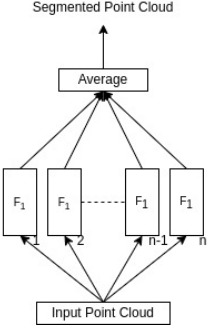
\includegraphics[scale=0.45]{images/flipout.jpg}
                \caption{Illustration of test dataflow in Flipout. Here $F_1$ represents the Flipout trained model and we
                compute n forward passes of the same point cloud on $F_1$.}
                \label{fig:flipout_work}
            \end{figure}
        \end{column}
    \end{columns}
\end{frame}
\begin{frame}[noframenumbering]{Setup}
    \begin{itemize}
        
        \item \textcolor{gray}{3D Semantic Segmentation model - RandLA-Net}
        \item \textcolor{gray}{Uncertainty methods - Deep Ensembles \& Flipout}
        \item OOD score methods
        \item Datasets
    \end{itemize}
\end{frame}
\begin{frame}{OOD Score calculation}
    \begin{itemize}
        \item We use the following two methods to generate the OOD scores.
        \item Maximum Softmax Probability
        \begin{itemize}
            \item $max(y_n), y_n = [P(C_1), P(C_2), ..., P(C_n)]$
        \end{itemize}
        \item Entropy
        \begin{itemize}
            \item $-\sum_i P(x_i)log(P(x_i))$ with $i$ iterates across all the classes for point $x$
        \end{itemize}
    \end{itemize}
\end{frame}
\begin{frame}[noframenumbering]{Setup}
    \begin{itemize}
        \item \textcolor{gray}{3D Semantic Segmentation model - RandLA-Net}
        \item \textcolor{gray}{Uncertainty methods - Deep Ensembles \& Flipout}
        \item \textcolor{gray}{OOD score methods - Maximum Softmax Probability \& Entropy}
        \item Datasets
    \end{itemize}
\end{frame}

\begin{frame}{3D LiDAR datasets}
    \begin{figure}
        \centering
        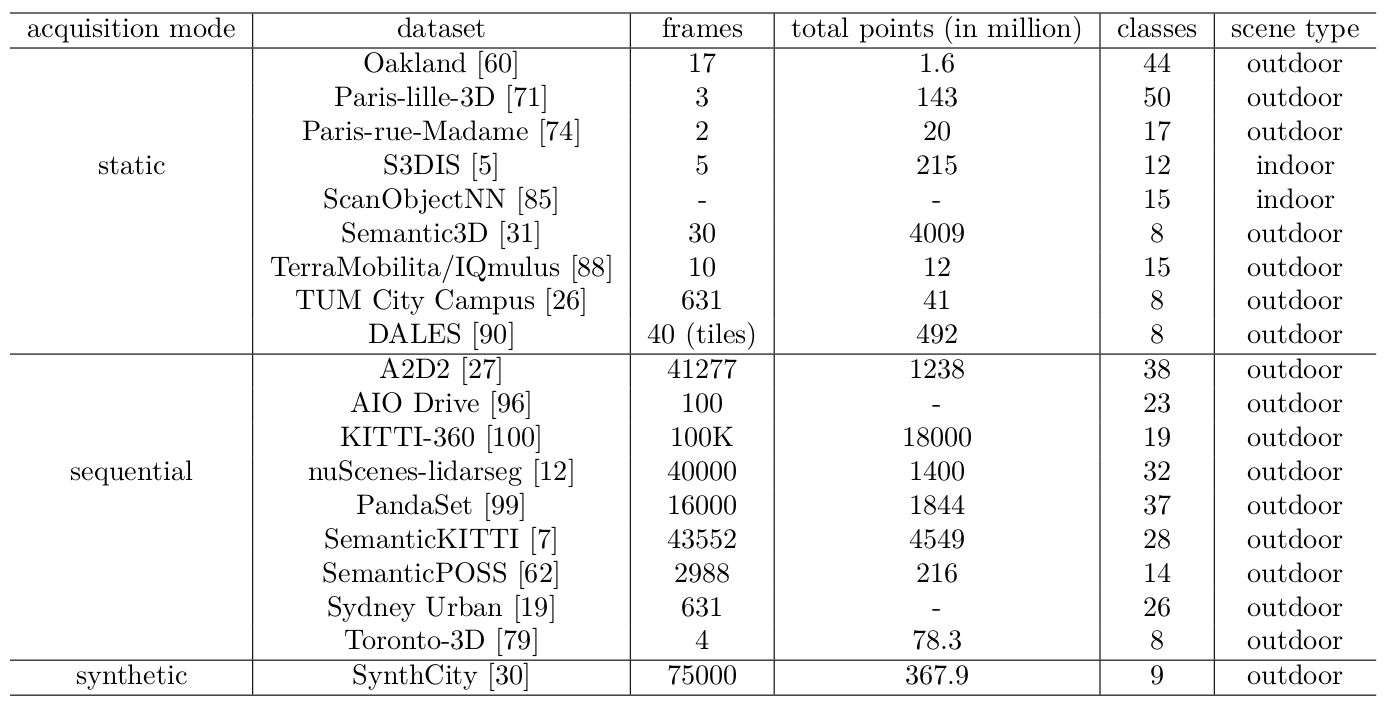
\includegraphics[scale=0.23]{images/sota_datasets.png}
    \end{figure}
    \begin{table}
        \caption{3D LiDAR datasets classified based on the acquisition type. Table updated from \cite{survey3d}.}
    \end{table}
\end{frame}
\begin{frame}{Semantic3D}
    \begin{columns}
        \begin{column}{0.5\textwidth}
            \begin{itemize}
                \item Huge 3D point cloud benchmark classification static dataset with 4 million points
                \item Scenes are taken in european streets around church, stations and fields
                \item Point features include XYZ, RGB and Intensity values.
                \item It has 8 classes with distribution of points represented in Figure~\ref{fig:sem3d_stats}
                \item \cite{hackel2017semantic3d} states that the scanning artefacts, hardscapes and cars are the most challenging classes
            \end{itemize}
        \end{column}
        \begin{column}{0.5\textwidth}
            \begin{figure}
                \centering
                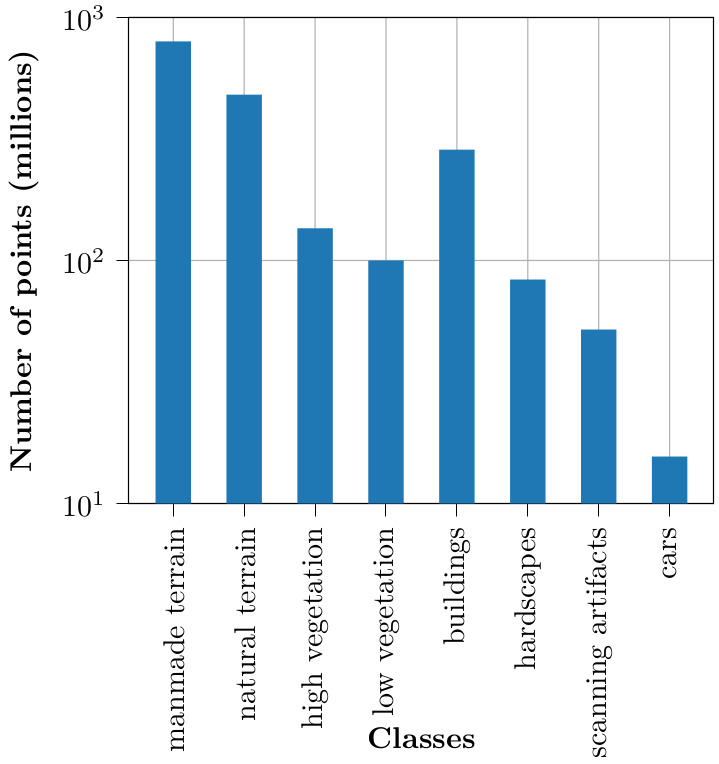
\includegraphics[scale=0.22]{images/sem3d/sem3d_stats.jpg}
                \caption{Graph depicting the number of points per class (in millions) in the Semantic3D dataset.}
                \label{fig:sem3d_stats}
            \end{figure}
        \end{column}
    \end{columns}
\end{frame}
\begin{frame}{Semantic3D}
    \begin{columns}
        \begin{column}{0.33\textwidth}
            \begin{figure}
                \centering
                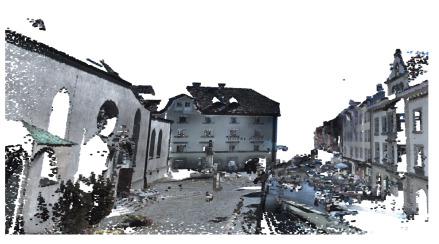
\includegraphics[scale=0.33]{images/sem3d/sem3d_sample_1.jpg}
                %\caption{caption}
                %\label{fig:sem3d_sample_1}    
            \end{figure}
        \end{column}
        \begin{column}{0.33\textwidth}
            \begin{figure}
                \centering
                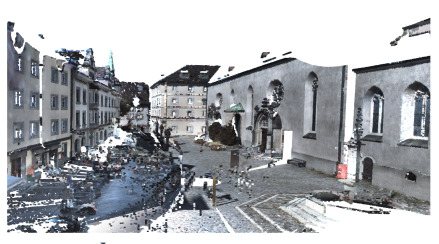
\includegraphics[scale=0.33]{images/sem3d/sem3d_sample_2.jpg}   
            \end{figure}
        \end{column}
        \begin{column}{0.33\textwidth}
            \begin{figure}
                \centering
                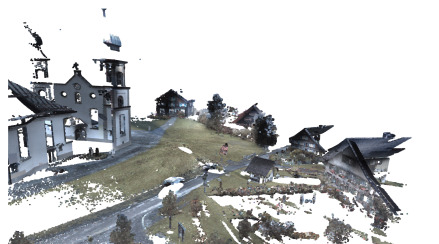
\includegraphics[scale=0.33]{images/sem3d/sem3d_sample_3.jpg}
                %\caption{caption}
                %\label{fig:sem3d_sample_3}    
            \end{figure}
        \end{column}
    \end{columns}
    \begin{figure}
        \centering
        \caption{Illustration of the Semantic3D point clouds of various outdoor scenes. Dataset from \cite{hackel2017semantic3d}.}
    \end{figure}
\end{frame}
\begin{frame}{S3DIS}
    \begin{columns}
        \begin{column}{0.6\textwidth}
            \begin{itemize}
                \item Indoor dataset with scans from various buildings
                \item Dataset include scans of personal offices, restrooms, open spaces, lobbies and hallways
                \item It has 12 classes, further subdivided into two types
                \begin{itemize}
                    \item structural elements 
                    \item everyday items
                \end{itemize}
                \item One of the most evaluated datasets for indoor semantic segmentation
            \end{itemize}
        \end{column}
        \begin{column}{0.4\textwidth}
            \begin{figure}
                \centering
                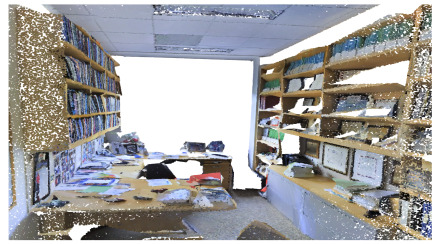
\includegraphics[scale=0.35]{images/s3dis/s3dis_sample_1.jpg}
                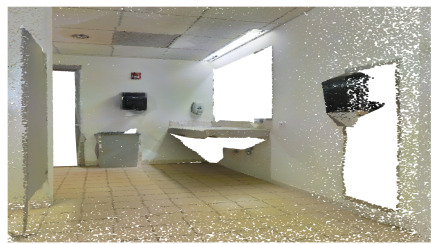
\includegraphics[scale=0.35]{images/s3dis/s3dis_sample_2.jpg}
                \caption{Illustration of the S3DIS point clouds of various indoor scenes. Dataset from \cite{Armeni_2016_CVPR_S3DIS}.}
                \label{fig:s3dis_sample_images}
            \end{figure}
        \end{column}
    \end{columns}
\end{frame}
\begin{frame}{OOD Benchmark datasets}
    %\begin{figure}
    %    \centering
    %    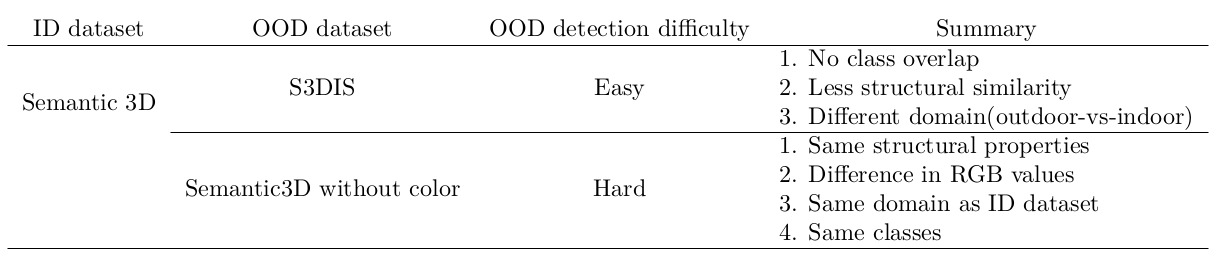
\includegraphics[scale=0.33]{images/benchmark_table.jpg}
    %\end{figure}
    %\begin{table}
    %    \caption{Table representing the ID dataset and corresponding OOD datasets, difficulty in OOD detection
    %    and the summary of reasons to chose this OOD dataset.}
    %\end{table}
    \begin{table}[h!]
        \resizebox{\textwidth}{!}{%
        \begin{tabular}{cccc}
        ID dataset                   & OOD dataset          &  OOD detection difficulty  & Summary                                                                                                                                                                             \\ \hline
        \multirow{2}{*}{Semantic 3D} & S3DIS                & Easy    & \multicolumn{1}{l}{\begin{tabular}[c]{@{}l@{}}$\bullet$ No class overlap\\ $\bullet$ Less structural similarity\\ $\bullet$ Different domain(outdoor-vs-indoor)\end{tabular}} \\ \cline{2-4} 
                                     & Semantic3D without colour & Hard & \multicolumn{1}{l}{\begin{tabular}[c]{@{}l@{}}$\bullet$ Same structural properties\\ $\bullet$ Difference in RGB values\\ $\bullet$ Same domain as ID dataset\\ $\bullet$ Same classes\end{tabular}}     \\ \hline
                                                                                                                                                                                       
        \end{tabular}
        }
        \caption{Table representing the ID dataset and corresponding OOD datasets, difficulty in OOD detection and the summary of reasons to chose this OOD dataset.}
        \label{tab:OOD_reasons}
        \end{table}
\end{frame}
\begin{frame}[noframenumbering]{Setup}
    \begin{itemize}
        \item 3D Semantic Segmentation model - RandLA-Net
        \item Uncertainty methods - Deep Ensembles \& Flipout
        \item OOD score methods - Maximum Softmax Probability \& Entropy
        \item Datasets - Semantic3D-vs-S3DIS \& Semantic3D-vs-Semantic3D without colour
    \end{itemize}
\end{frame}
%%%%%%%%%%%%%%%%%%%%%%%%%%%%%%%%%%%%%%%%%%%%%%%%%%%%%%%%%%%%%%%%%%%%%%%%%%%%%%%%%%%%%%%%
%%%%%%%%%%%%%%%%%%%%%%%        Experiments          %%%%%%%%%%%%%%%%%%%%%%%%%%%%%%%%%%%%
%%%%%%%%%%%%%%%%%%%%%%%%%%%%%%%%%%%%%%%%%%%%%%%%%%%%%%%%%%%%%%%%%%%%%%%%%%%%%%%%%%%%%%%%
\section{Experiments \& Results}
\begin{frame}[noframenumbering]{Experiments}
    \begin{itemize}
        \item Semantic3D-vs-S3DIS
        \begin{itemize}
            \item Deep Ensembles
            \item Flipout
            \item Area Under Receiver Operating Characteristic (AUROC) score comparison
        \end{itemize}
        \item Semantic3D-vs-Semantic3D without colour
    \end{itemize}
\end{frame}
\begin{frame}{Semantic3D-vs-S3DIS - Deep Ensembles}
    \begin{figure}
        \centering
        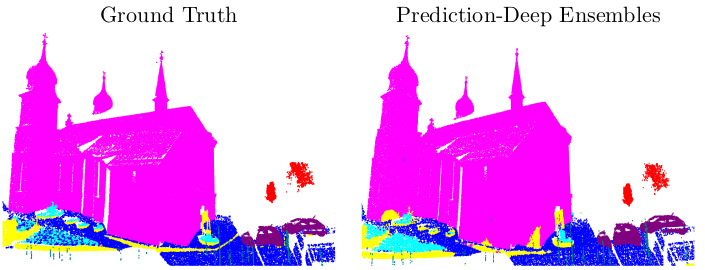
\includegraphics[scale=0.5]{images/sem3d/Sem3d_DE_output.jpg}
        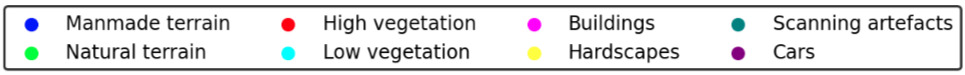
\includegraphics[scale=0.25]{images/legend.jpg}
        \caption{Image representing the predictions (last column) from Deep Ensemble with an ensemble size
        of 15 on Semantic3D dataset. The first column depict the ground truth.}
        \label{fig:sem3d_de_op}
    \end{figure}
\end{frame}
\begin{frame}{Semantic3D-vs-S3DIS - Deep Ensembles}
    \begin{figure}
        \centering
        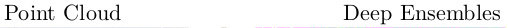
\includegraphics[scale=0.5]{images/s3dis/top_legend_s3dis_DE.jpg}
        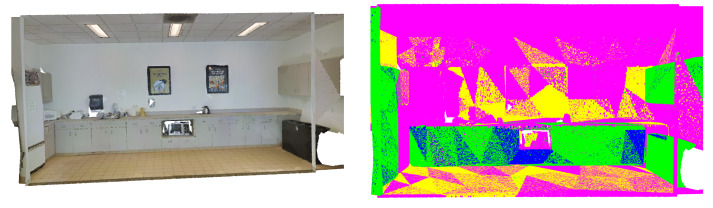
\includegraphics[scale=0.5]{images/s3dis/S3DIS_DE_output.jpg}
        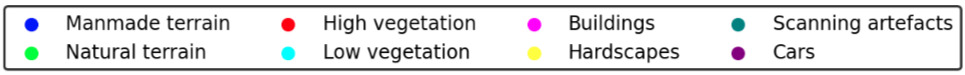
\includegraphics[scale=0.25]{images/legend.jpg}
        \caption{Predictions of RandLA-Net on S3DIS (OOD) dataset. First column representing the point
        cloud, second column presenting the predictions of Deep Ensembles (15 Ensemble size).}
        \label{fig:s3dis_de_op}
    \end{figure}
\end{frame}
\begin{frame}{Semantic3D-vs-S3DIS - Deep Ensembles}
    \begin{columns}
        \begin{column}{0.5\textwidth}
            \begin{figure}
                \centering
                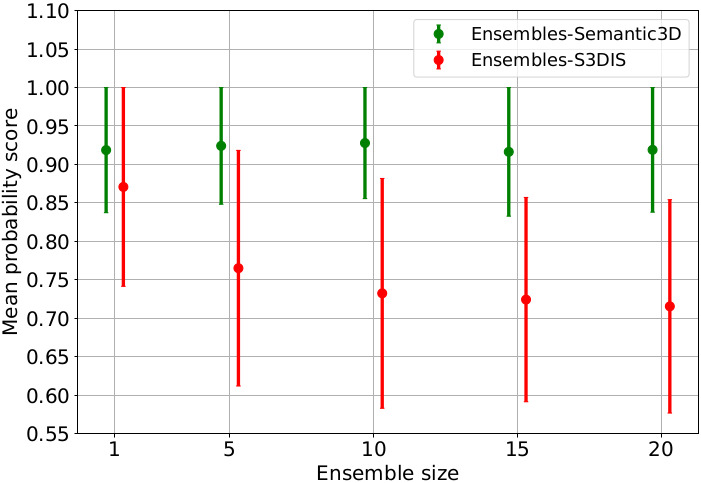
\includegraphics[scale=0.28]{images/ood1/MSP_Mean_OOD1_DE.jpg}
            \end{figure}
        \end{column}
        \begin{column}{0.5\textwidth}
            \begin{figure}
                \centering
                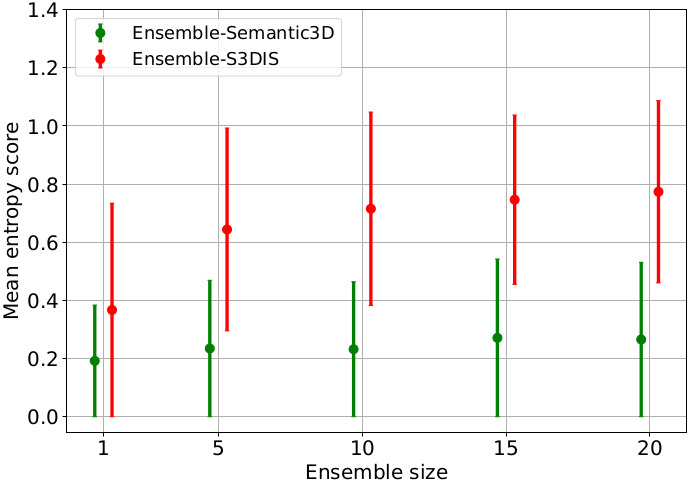
\includegraphics[scale=0.28]{images/ood1/Ent_Mean_OOD1_DE.jpg}
            \end{figure}
        \end{column}
    \end{columns}
    \begin{figure}
        \caption{Graphs representing the mean probability value and mean entropy as a dot for Semantic3D (ID) in green and
        S3DIS (OOD) in red when using Deep Ensembles. The variance is represented via the error bars.}
    \end{figure}
\end{frame}

\begin{frame}{Semantic3D-vs-S3DIS - Flipout}
    \begin{figure}
        \centering
        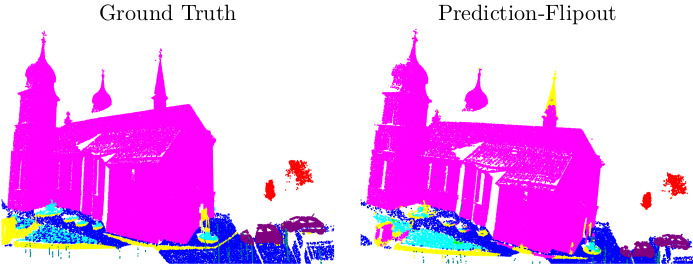
\includegraphics[scale=0.5]{images/sem3d/Sem3d_Fout_op.jpg}
        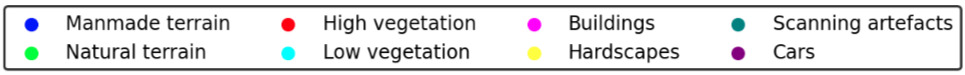
\includegraphics[scale=0.25]{images/legend.jpg}
        \caption{Image representing the predictions (last column) from Flipout with 15 number of passes on Semantic3D dataset. The first column depict the ground truth.}
        \label{fig:sem3d_fout_op}
    \end{figure}
\end{frame}
\begin{frame}{Semantic3D-vs-S3DIS - Flipout}
    \begin{columns}
        \begin{column}{0.5\textwidth}
            \begin{figure}
                \centering
                
\includegraphics[scale=0.5]{images/s3dis/s3dis_fout_orig_head.png}
                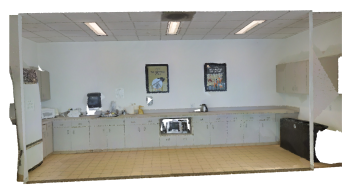
\includegraphics[scale=0.5]{images/s3dis/s3dis_fout_orig.png}
            \end{figure}
        \end{column}
        \begin{column}{0.5\textwidth}
            \begin{figure}
                \centering
                
\includegraphics[scale=0.5]{images/s3dis/s3dis_fout_semseg_head.png}
                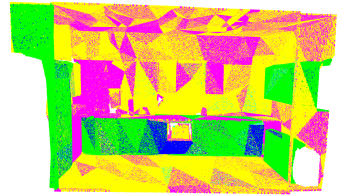
\includegraphics[scale=0.5]{images/s3dis/s3dis_fout_semseg.png}
            \end{figure}
        \end{column}
    \end{columns}
    \begin{figure}
        \centering
        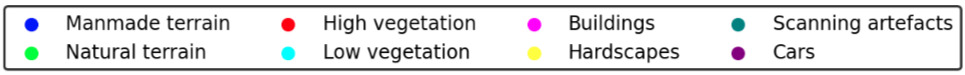
\includegraphics[scale=0.25]{images/legend.jpg}
        \caption{Predictions of RandLA-Net on S3DIS (OOD) dataset. First column representing the point
        cloud, second column presenting the predictions from Flipout (15 number of passes).}
    \end{figure}
\end{frame}
\begin{frame}{Semantic3D-vs-S3DIS - Flipout}
    \begin{columns}
        \begin{column}{0.5\textwidth}
            \begin{figure}
                \centering
                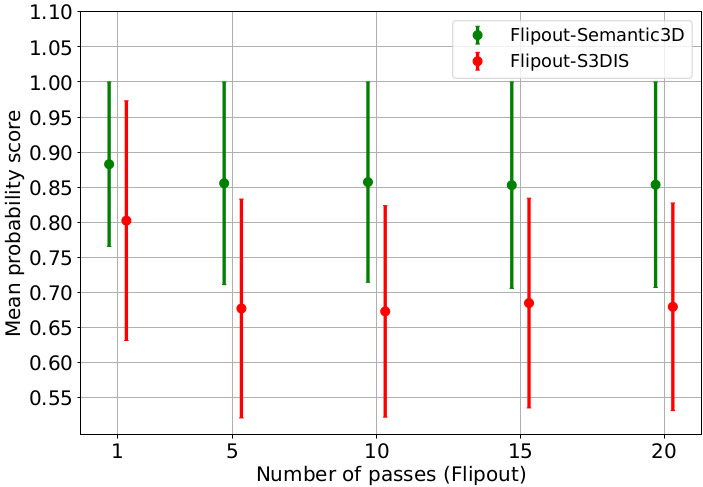
\includegraphics[scale=0.28]{images/ood1/MSP_Mean_OOD1_Fout.jpg}
            \end{figure}
        \end{column}
        \begin{column}{0.5\textwidth}
            \begin{figure}
                \centering
                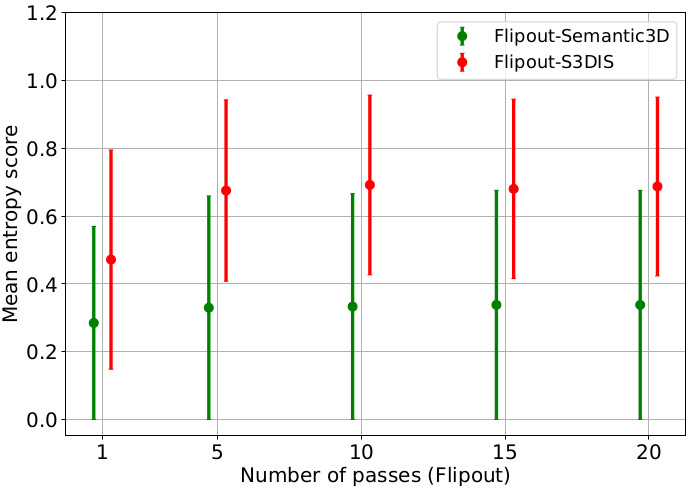
\includegraphics[scale=0.28]{images/ood1/Ent_Mean_OOD1_Fout.jpg}
            \end{figure}
        \end{column}
    \end{columns}
    \begin{figure}
        \caption{Graphs representing the mean probability value and mean entropy as a dot for Semantic3D (ID) in green and
        S3DIS (OOD) in red when using Flipout. The variance is represented via the error bars.}
    \end{figure}
\end{frame}
\begin{frame}{Semantic3D-vs-S3DIS - AUROC Scores}
            %\begin{figure}
            %    \centering
            %    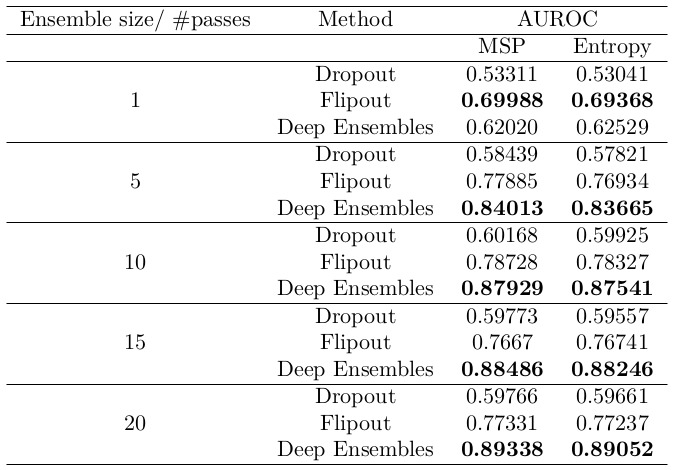
\includegraphics[scale=.33]{images/ood1/AUROC_OOD1_Scores.jpg}
            %\end{figure}   
            %\begin{table}
            %    \caption{AUROC scores calculated for all the points in the test sets of Semantic3D and S3DIS for
            %    Dropout, Flipout, and Deep Ensembles generated using MSP and entropy values for various ensemble
            %    sizes and forward passes.}
            %\end{table}
            \begin{table}[h!]
                \resizebox{\textheight}{!}{%
                \centering
                \begin{tabular}{cccc}
                \hline
                Ensemble size/ \#passes & Method               &  \multicolumn{2}{c}{AUROC}          \\ \hline
                                        &                      &  MSP              & Entropy         \\ \hline
                \multirow{3}{*}{1}      & Dropout              & 0.53311          & 0.53041          \\
                                        & Flipout              & \textbf{0.69988} & \textbf{0.69368} \\
                                        & Deep Ensembles       & 0.62020          & 0.62529          \\ \hline
                \multirow{3}{*}{5}      & Dropout              & 0.58439          & 0.57821          \\
                                        & Flipout              & 0.77885          & 0.76934          \\
                                        & Deep Ensembles       & \textbf{0.84013} & \textbf{0.83665} \\ \hline
                \multirow{3}{*}{10}     & Dropout              & 0.60168          & 0.59925          \\
                                        & Flipout              & 0.78728          & 0.78327          \\
                                        & Deep Ensembles       & \textbf{0.87929} & \textbf{0.87541} \\ \hline
                \multirow{3}{*}{15}     & Dropout              & 0.59773          & 0.59557          \\
                                        & Flipout              & 0.7667           & 0.76741          \\
                                        & Deep Ensembles       & \textbf{0.88486} & \textbf{0.88246} \\ \hline
                \multirow{3}{*}{20}     & Dropout              & 0.59766          & 0.59661          \\
                                        & Flipout              & 0.77331          & 0.77237          \\
                                        & Deep Ensembles       & \textbf{0.89338} & \textbf{0.89052} \\ \hline
                \end{tabular}
                }
                \caption{AUROC scores calculated for all the points in the test sets of Semantic3D and S3DIS for Dropout, Flipout, and  Deep Ensembles generated using MSP and entropy values for various ensemble sizes and forward passes.}
                \label{tab:sem3dvs3dis_auroc}
            \end{table}
\end{frame}
\begin{frame}{Semantic3D-vs-S3DIS - AUROC Scores}
    \begin{figure}
        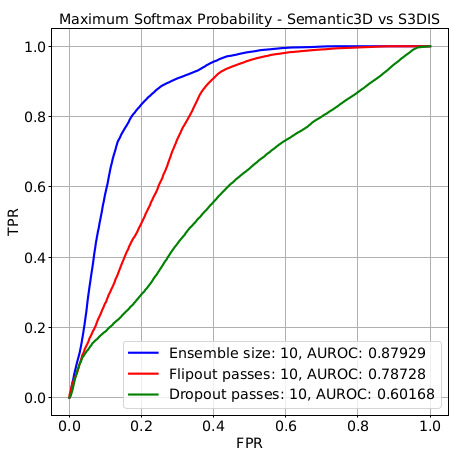
\includegraphics[scale = 0.35]{images/ood1_msp_roc.jpg}
        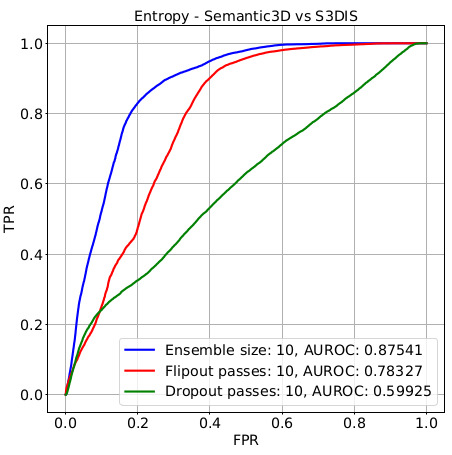
\includegraphics[scale=0.35]{images/ood1_ent_roc.jpg}
        \caption{ROC curves of Semantic3D-vs-S3DIS for 10 Ensembles, 10 forward passes for Flipout and
        Dropout using Maximum Softmax Probability and Entropy respectively.}
    \end{figure}
\end{frame}



%%%%%%%%%%%%%%%%%%%%%%%%%%%%%%%%%%%%%%%%%%%%%%%%%%%%%%%%%%%%%%%%%%%%%%%%%%%%%%%%%%%%%%%%
%%%%%%%%%%%%%%%%%%%%%%%        Experiment2           %%%%%%%%%%%%%%%%%%%%%%%%%%%%%%%%%%%
%%%%%%%%%%%%%%%%%%%%%%%%%%%%%%%%%%%%%%%%%%%%%%%%%%%%%%%%%%%%%%%%%%%%%%%%%%%%%%%%%%%%%%%%
\begin{frame}[noframenumbering]{Experiments}
    \begin{itemize}
        \item \textcolor{gray}{Semantic3D-vs-S3DIS}
        
        \item Semantic3D-vs-Semantic3D without colour
        \begin{itemize}
            \item Deep Ensembles
            \item Flipout
            \item Area Under Receiver Operating Characteristic (AUROC) score comparison
        \end{itemize}
    \end{itemize}
\end{frame}
\begin{frame}{Semantic3D colour-vs-without colour - Deep Ensembles}
    \begin{figure}
        \centering
        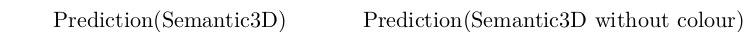
\includegraphics[scale=0.5]{images/ood2/top_legend_ood2.jpg}
        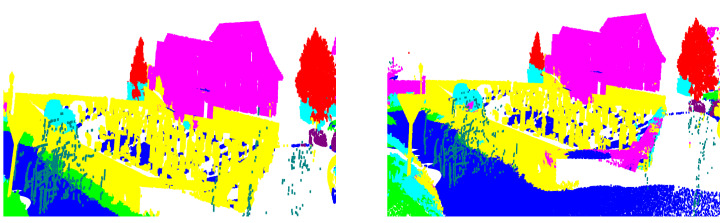
\includegraphics[scale=0.5]{images/ood2/Sem3d_OOD2_DE.jpg}
        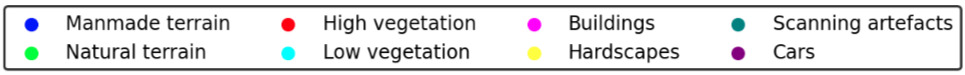
\includegraphics[scale=0.25]{images/legend.jpg}
        \caption{Output predictions of the RandLA-Net over the Semantic3D dataset and Semantic3D without
        colour dataset using Deep Ensembles (Ensemble size of 10).}
        \label{fig:DE_ood2_op}
    \end{figure}
\end{frame}
\begin{frame}{Semantic3D colour-vs-without colour - Deep Ensembles}
    \begin{columns}
        \begin{column}{0.5\textwidth}
            \begin{figure}
                \centering
                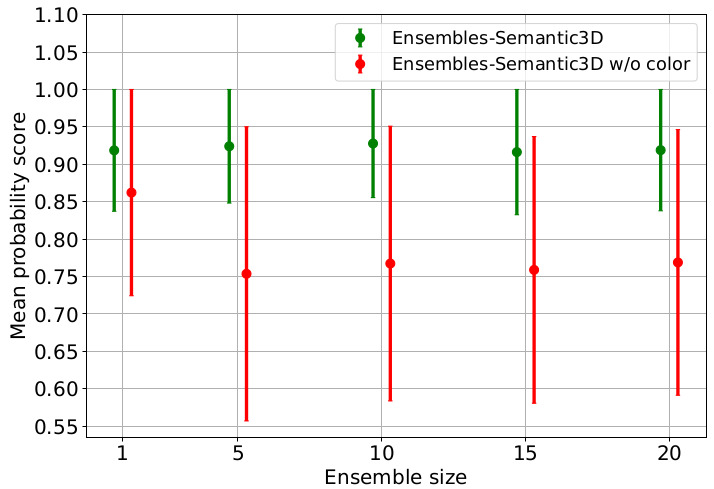
\includegraphics[scale=0.25]{images/ood2/DE_MSP_OOD2.jpg}
            \end{figure}
        \end{column}
        \begin{column}{0.5\textwidth}
            \begin{figure}
                \centering
                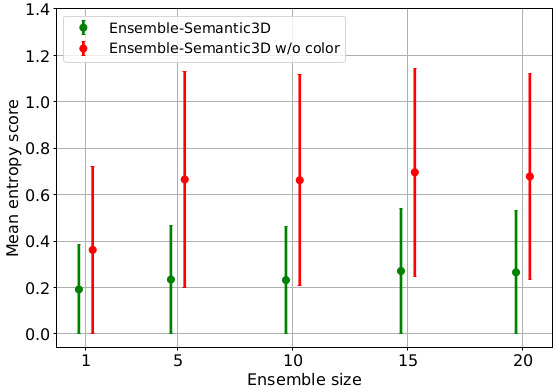
\includegraphics[scale=0.32]{images/ood2/DE_Ent_OOD2.jpg}
            \end{figure}
        \end{column}
    \end{columns}
    \begin{figure}
        \caption{Graphs representing the mean probability value and mean entropy as a dot for Semantic3D (ID) in green and
        Semantic3D without colour (OOD) in red when using Deep Ensembles. The variance is represented via the error bars.}
    \end{figure}
\end{frame}

%\begin{frame}{Semantic3D colour-vs-without colour - Flipout}
%    \begin{figure}
%        \centering
%        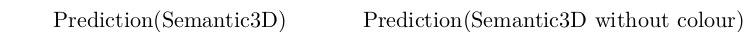
\includegraphics[scale=0.5]{images/ood2/top_legend_ood2.jpg}
%        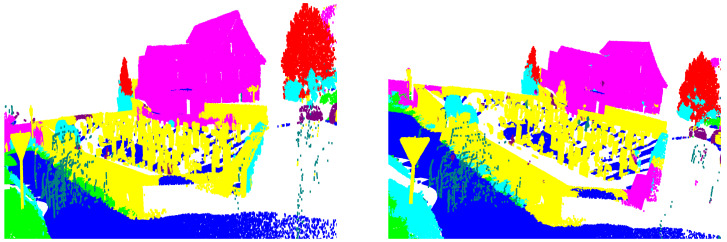
\includegraphics[scale=0.5]{images/ood2/Sem3d_OOD2_Fout.jpg}
%        \caption{caption}
%        \label{fig:Fout_ood2_op}
%    \end{figure}
%\end{frame}
\begin{frame}{Semantic3D colour-vs-without colour - Flipout}
    \begin{columns}
        \begin{column}{0.5\textwidth}
            \begin{figure}
                \centering
                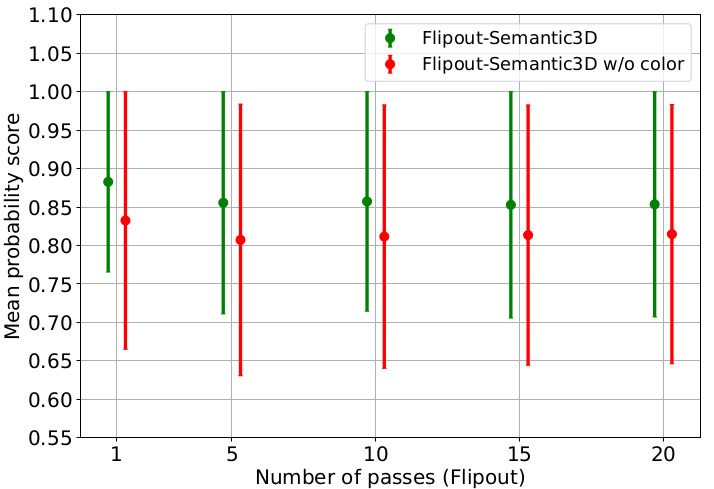
\includegraphics[scale=0.25]{images/ood2/Fout_MSP_OOD2.jpg}
            \end{figure}
        \end{column}
        \begin{column}{0.5\textwidth}
            \begin{figure}
                \centering
                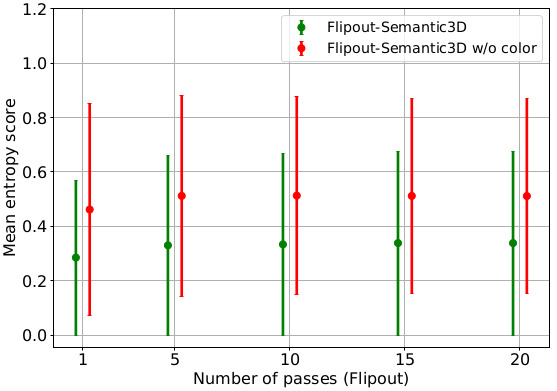
\includegraphics[scale=0.32]{images/ood2/Fout_Ent_OOD2.jpg}
            \end{figure}
        \end{column}
    \end{columns}
    \begin{figure}
        \caption{Graphs representing the mean probability value and mean entropy as a dot for Semantic3D (ID) in green and
        Semantic3D without colour (OOD) in red when using Flipout. The variance is represented via the error bars.}
    \end{figure}
\end{frame}

\begin{frame}{Semantic3D colour-vs-without colour - AUROC Scores}
    %\begin{figure}
    %    \centering
    %    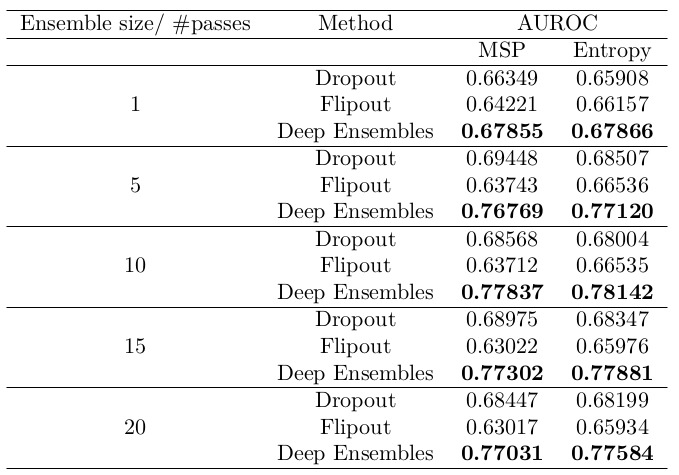
\includegraphics[scale=0.33]{images/ood2/AUROC_OOD2.jpg}
    %\end{figure}
    %\begin{table}
    %    \caption{AUROC scores in case of Semantic3D-vs-Semantic3D without colour for Dropout, Flipout, and
    %    Deep Ensembles generated using MSP and entropy values for various ensemble sizes and forward passes.}
    %\end{table}
    \begin{table}[h!]
        \resizebox{0.8\textheight}{!}{%
        \centering
        \begin{tabular}{cccc}
        \hline
        Ensemble size/ \#passes & Method               &  \multicolumn{2}{c}{AUROC}          \\ \hline
                                &                      &  MSP             & Entropy          \\ \hline
        \multirow{3}{*}{1}      & Dropout              & 0.66349          & 0.65908          \\
                                & Flipout              & 0.64221          & 0.66157          \\
                                & Deep Ensembles       & \textbf{0.67855} & \textbf{0.67866} \\ \hline
        \multirow{3}{*}{5}      & Dropout              & 0.69448          & 0.68507          \\
                                & Flipout              & 0.63743          & 0.66536          \\
                                & Deep Ensembles       & \textbf{0.76769} & \textbf{0.77120} \\ \hline
        \multirow{3}{*}{10}     & Dropout              & 0.68568          & 0.68004          \\
                                & Flipout              & 0.63712          & 0.66535          \\
                                & Deep Ensembles       & \textbf{0.77837} & \textbf{0.78142} \\ \hline
        \multirow{3}{*}{15}     & Dropout              & 0.68975          & 0.68347          \\
                                & Flipout              & 0.63022           & 0.65976          \\
                                & Deep Ensembles       & \textbf{0.77302} & \textbf{0.77881} \\ \hline
        \multirow{3}{*}{20}     & Dropout              & 0.68447          & 0.68199          \\
                                & Flipout              & 0.63017          & 0.65934          \\
                                & Deep Ensembles       & \textbf{0.77031} & \textbf{0.77584} \\ \hline
        \end{tabular}
        }
        \caption{AUROC scores in case of Semantic3D-vs-Semantic3D without colour for Dropout, Flipout, and  Deep Ensembles generated using MSP and entropy values for various ensemble sizes and forward passes.}
        \label{tab:auroc_ood_2}
    \end{table}
\end{frame}
\begin{frame}{Semantic3D colour-vs-without colour - AUROC Scores}
    \begin{figure}
        \centering
        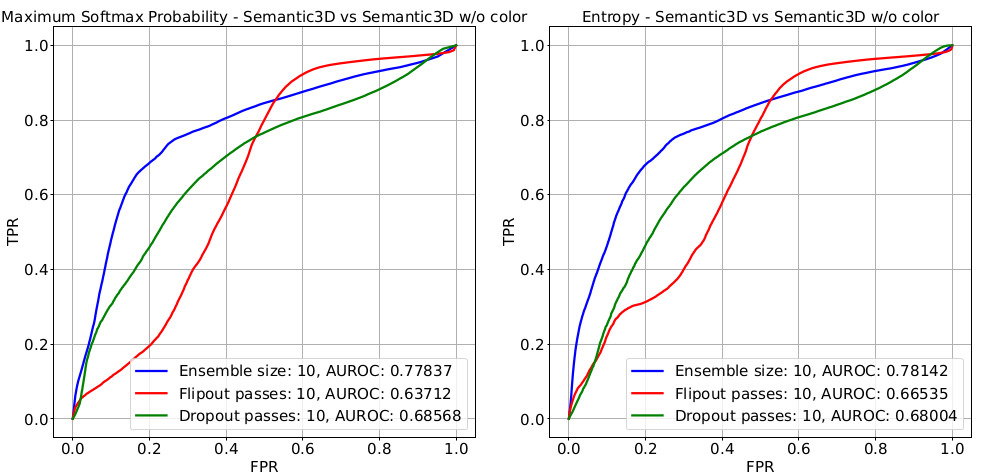
\includegraphics[scale=0.3]{images/ood2_roc_curves.jpg}
        \caption{ROC curves of Semantic3D-vs-Semantic3D without colour for 10 ensembles, 10 forward
        passes for Flipout and Dropout using Maximum Softmax Probability and Entropy scores respectively.}
    \end{figure}
\end{frame}

% Arrange the experiments and explain the results here
%%%%%%%%%%%%%%%%%%%%%%%%%%%%%%%%%%%%%%%%%%%%%%%%%%%%%%%%%%%%%%%%%%%%%%%%%%%%%%%%%%%%%%%%
%%%%%%%%%%%%%%%%%%%%%%%        Conclusion         %%  %%%%%%%%%%%%%%%%%%%%%%%%%%%%%%%%%%
%%%%%%%%%%%%%%%%%%%%%%%%%%%%%%%%%%%%%%%%%%%%%%%%%%%%%%%%%%%%%%%%%%%%%%%%%%%%%%%%%%%%%%%%
\section{Conclusion}
\begin{frame}{Conclusion}
    \begin{itemize}
        \item We propose two benchmark datasets 
        \begin{itemize}
            \item Semantic3D-vs-S3DIS (Outdoor-vs-Indoor) - Easy OOD identification
            \item Semantic3D-vs-Semantic3D without colour - Hard OOD identification
        \end{itemize}
        \item The second case is hard because of same point geometry between ID and OOD datasets
        \item Both Maximum Softmax Probability and Entropy are able to identify OOD points
        \item Deep Ensembles outperform Flipout and Dropout in both the benchmark datasets
    \end{itemize}
\end{frame}
\begin{frame}{Lessons Learned}
    \begin{itemize}
        \item Training and evaluation of 3D DNNs are time-consuming and resource-intensive.
        \item Finding the proper prior for Flipout layers is hard and currently we use brute force to find the best fitting prior.
        %\item OOD benchmarking require in depth analysis of datasets like studying the structural similarties in the datasets and also colour spectrum.
        \item LiDAR datasets have large memory requirements especially for preprocessing and metric computation.
        \item Getting 100\% OOD detection performance is not possible with the post-hoc methods used as some points in the ID dataset also have low probability scores.
    \end{itemize}
\end{frame}
\begin{frame}{Future Work}
    \begin{itemize}
        \item This thesis is limited to only point-based models, this can be extended to graph and projection-based models.
        \item The datasets involved are only static datasets and this thesis study can be further extended to other type of datasets such as synthetic and sequential datasets.
        \item Since this thesis utilizes post-hoc threshold methods for OOD detection. Other methods such as Mahalanobis distance-based OOD detection \cite{lee2018simple_mahalanobis} or MetaSeg \cite{MetaSeg} can be added as an extension to this thesis.
    \end{itemize}
\end{frame}
%%%%%%%%%%%%%%%%%%%%%%%%%%%%%%%%%%%%%%%%%%%%%%%%%%%%%%%%%%%%%%%%%%%%%%%%%%%%%%%%%%%%%%%%
%%%%%%%%%%%%%%%%%%%%%%%        References%%           %%%%%%%%%%%%%%%%%%%%%%%%%%%%%%%%%%
%%%%%%%%%%%%%%%%%%%%%%%%%%%%%%%%%%%%%%%%%%%%%%%%%%%%%%%%%%%%%%%%%%%%%%%%%%%%%%%%%%%%%%%%

\begin{frame}[noframenumbering, allowframebreaks]{References}
    \bibliographystyle{plain}
    \bibliography{bibliography.bib}

\end{frame}
%%%%%%%%%%%%%%%%%%%%%%%%%%%%%%%%%%%%%%%%%%%%%%%%%%%%%%%%%%%%%%%%%%%%%%%%%%%%%%%%%%%%%%%%
%%%%%%%%%%%%%%%%%%%%%%%        Extra slides           %%%%%%%%%%%%%%%%%%%%%%%%%%%%%%%%%%
%%%%%%%%%%%%%%%%%%%%%%%%%%%%%%%%%%%%%%%%%%%%%%%%%%%%%%%%%%%%%%%%%%%%%%%%%%%%%%%%%%%%%%%%

\begin{frame}[noframenumbering]{What is OOD Detection?}
    \begin{figure}
        \centering
        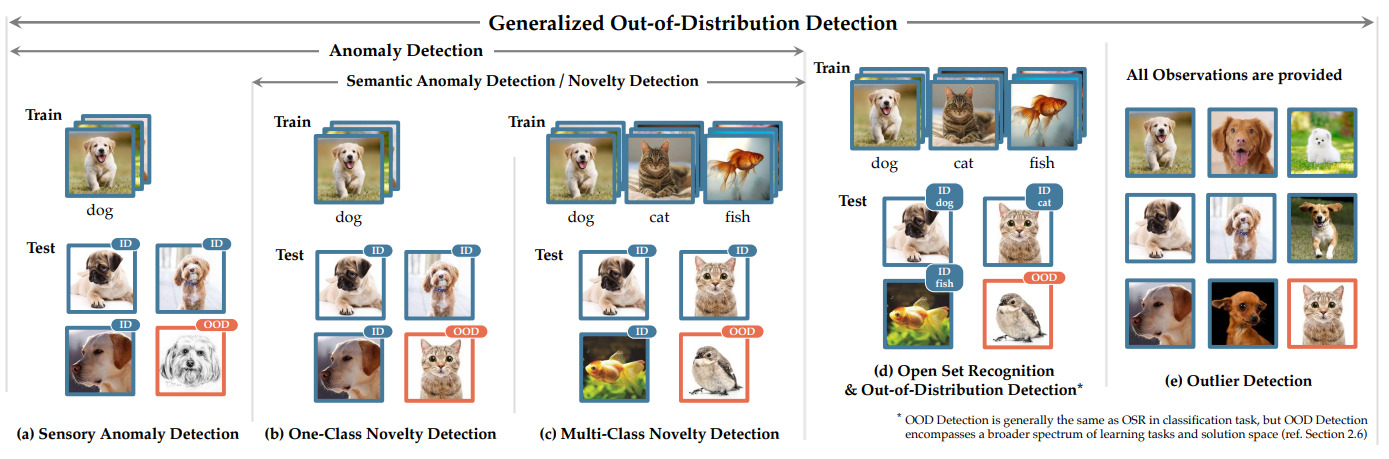
\includegraphics[scale=0.3]{images/OOD_ex_new.jpg}
        \caption{Generalized Out-of-Distribution Detection: A Survey}
        \label{fig:my_label}
    \end{figure}
\end{frame}

\begin{frame}[noframenumbering]{Semantic3D-Deep Ensembles}
    \begin{figure}
        \centering
        \includegraphics[scale=0.4]{images/Semantic3d_DE.jpg}
    \end{figure}
\end{frame}
\begin{frame}[noframenumbering]{Semantic3D-Flipout}
    \begin{figure}
        \centering
        \includegraphics[scale=0.4]{images/Semantic3d_Fout.jpg}
    \end{figure}
\end{frame}
\end{document}

